
\documentclass[12pt, man, natbib]{apa6}
\usepackage[USenglish]{babel}
\usepackage{setspace}
\usepackage{hyperref}

\title{A Couple of Spills a Year, That's Normal? Learning and Greenwashing in the Pipeline Industry}
\shorttitle{Thesis Proposal -- Julian Barg}
\author{Julian Barg\\jbarg.phd@ivey.ca}
\affiliation{Ivey Business School}
\setcitestyle{authoryear, open={()},close={)},citesep={,},aysep=}
\abstract{
	From 2000 to 2020, the standardized spill volume of refined petroleum pipelines has stayed constant at about 15 bbl per billion barrel-miles transported. In contrast, from 1980 to 2000, standardized spill volume had about halved. This dissertation researches why pipeline operators in the US keep causing and getting away with pipeline spills. The dissertation uses two lenses, organizational learning and greenwashing. These lenses reveal why, despite continuous efforts by engineers, the safety record of the industry has stagnated. The learning literature suggests that it is commonplace for organizational learning to converge at a high level of performance, as observed in the pipeline industry. Greenwashing is a strategy for organizations to escape negative consequences for poor environmental performance.
	
	The first chapter reveals the mechanisms behind the convergence in organizational learning. The empirical section uses a dataset of 6,147 pipeline spills, and qualitative data on 10 significant pipeline spill. This research reveals that valid learning only occurs in response to the spills that an operator experiences. For a general theory of learning, the empirical findings suggests that learning converges when the organization or system that learns has developed a high degree of complexity. Because of this complexity, learning in response to triggers such as failures is not sufficient anymore for making aggregate improvements. Learning turns into a perpetual game of whack-a-mole.
	
	The second chapter takes an encompassing look at the learning literature and promotes a more universal, new theory on the validity and reliability of learning. When learning goes beyond incremental improvements and touches on fundamental assumptions, organizations or industries can break out of their trajectory. However, many learning outcomes that have been thought of as "breakthroughs" have not led to the promised revolutions in the market. Validity and reliability fill an important gap in the literature of learning: even when learning produces sensible and internally consistent insights, these insights are meaningless if they do not serve for the organization to better understand, predict, and control existing problems, limitations, or bottlenecks--that is, if the knowledge is not valid. And valid knowledge still fails to make an impact if it is not reliable, meaning not shared across the organizational members who are to implement the insights.
	
	Finally, the third chapter discusses how pipeline operators keep in check the backlash for the environmental pollution that they cause. Pipeline operators shield themselves from criticism using new technology. When an operator causes a spill, the operator can point to the latest development in the constant flow of new technology as a remedy for future spills. The third chapter uses the same data on pipeline spills and pipeline networks as the first chapter, and adds text data from operators and industry level actors. I then track empirically how these patterns of greenwashing are diffused in the pipeline industry. This analysis sheds light on the role of industry level actors (such as the American Petroleum Institute) in greenwashing.
}

\keywords{organizational learning, greenwashing, industry level, population level, pipeline spills}

\begin{document}
	
	\maketitle
	
%	\singlespacing

	\tableofcontents
	
	\newpage
	
	\section{Introduction}

\begin{singlespace} 
	\begin{quote}
		"[T]here is perhaps an over-emphasis of technology in [Leak Detection Systems]. A recurring theme is that of false alarms. The implication is that [a Leak Detection System] is expected to perform as an elementary industrial automation alarm, with an on/off state and six-sigma reliability. Any alarm that does not correspond to an actual leak is, with this thinking, an indicator of a failure of the LDS system. Instead, multiple technical studies confirm that far more thought is required in dealing with leak alarms" -- \citet[p. 2-3]{Shaw2012}.
	\end{quote}
\end{singlespace}

How does an industry get stuck with a never-ending series of pollution events? It is the conventional view of organizational learning that performance measures, after initially exhibiting fast improvements, will settle at at a certain level \citep{Argote2013-1}. In other words, learning levels off. The \textit{organizational knowledge} view--the dominant stream of the learning literature--suggests that organizations accumulate knowledge which is held by individuals, in routines, or in transactive memory systems \citep{Bingham2011, Argote2011}. New knowledge is added to an existing "stock", presumably until there is no more new insights to be added. Disclosure of the outcomes of this learning process then is a subsequent, separate step--the organization makes a strategic decision as to which outcomes to share with stakeholders. To withhold negative information on environmental performance in this step would constitute greenwashing \citep{Lyon2011}.

An alternative view suggests that organizations can break out of existing trajectories and escape their constraints in learning--but that to do so requires a considerable rethinking of existing paradigms \citep{March2010}. For instance, an organization can reimagine how it measures performance \citep{Argyris1978}. This is consistent with the \textit{organizational routines} view, which holds that organizations develop not knowledge but patterns of action in stable environments \citep{Bingham2011}. The organizational routines view also postulates that in the absence of significant interventions, intricate but ultimately obsolete systems develop, for instance ones that rely on outdated technologies \citep{March1991}. With sufficient complexity, these systems can generate a never-ending stream of unexpected interactions and externalities, which then become relevant for sustainability research when the organization or industry has a catastrophic potential \citep{Perrow1984, Beck1992}. One would hope for stakeholders to be able to identify the pattern of unexpected interactions and externalities, but under an inadequate environmental regime the organization or industry can escape scrutiny through greenwashing \citep{Lyon2015}.

The inconsistent predictions of the two views, and their implications for persistent environmental pollution raises two questions. (1) \textit{How does the convergence of performance measures take place?} When the convergence has taken place in an organization or industry, do we see evidence for either the organizational knowledge or the organizational routines view? The organizational knowledge view suggests that once performance has converged, either no new knowledge is gained, or knowledge disappears at the same rate as it is produced \citep{Argote2013-3}. The organizational routines view makes no such prediction, instead, if that view was accurate we would see increasingly intricate routines with ultimately have little impact on performance. 

An obvious extension to the first question is a look at possibilities for organizations to break out of a state of convergence. The \textit{organizational routines} literature holds that organizations can break out of a state of convergence through what the \textit{organizational routines} literature calls either double-loop learning \citep{Argyris1978} or high-intellect learning \citep{March2010}. Two overlooked attributes of knowledge, \textit{validity} and \textit{reliability} could mend the split between the two streams of the organizational learning literature. \textit{Validity} describes whether knowledge does allow an organization to better understand, predict, and control problems, such as technological limitations or bottlenecks. \textit{Reliability} describes the degree to which member of the organization have command of the knowledge \citep{Rerup2020}. Validity and reliability allow for a critical view on the first question, and whether that state of convergence is inevitable.

(2) The state of convergence should be fairly obvious to stakeholders when environmental pollution is involved. The second research question addresses the difficulties that continuous environmental pollution would be expected to entail. \textit{How does an organization manage--or greenwash--its convergence to a state of constant pollution?} If the state of convergence is obvious for observers, one would expect calls for substantive change to be quite loud. But the pipeline industry has maintained the status quo for twenty years, which presumably requires an effort to maintain the status quo rather than just an absence of efforts to break out of the state of convergence.

%Learning is more complex than the existing view would suggest--organizations can leave an existing trajectory, but requires a considerable rethinking of existing paradigms \citep{Argyris1978, March2010, March1991}. An explanation for the divergence within the existing literature are two overlooked attributes of knowledge: validity and reliability \citep{Rerup2020}. The disclosure of information on environmental performance is closely related to the generation of knowledge and beliefs. The existing literature considers greenwashing to be a strategizing process that occurs when environmental outcomes are already determined \citep{Delmas2011}. Existing research on intra-industrial processes however suggest that information disclosure and the generation of new knowledge are closely related \citep{Maguire2009}. This dissertation deciphers the processes of knowledge creation, convergence of environmental performance, and greenwashing through two research questions. (1) \textit{How does an organization that effectively learns from failures also stagnate?} And (2) \textit{how does an industry greenwash its stagnatioinn in environmental performance?}

To answer the research questions, this dissertation employs data on the US pipeline industry. The pipeline industry offers an advantage over other industries with regard to studying environmental impacts, learning, and greenwashing, in that the industry's environmental pollution very much takes place in the public. Unlike other industries, pipeline spills do not occur inside private plants, locked away from the public eye. Pipeline spills usually occur on public land that the pipeline operator has only acquired the right-of-way of. Pipeline spills also receive a lot of attention from the press, government agencies, and environmental grassroot organizations. These actors pay particular attention to large pipeline spills, which make up for a majority of annual spill volume. Finally, the scrutiny of oil spills also ensures that the reported data is more accurate. Government-employed emergency responders are on site alongside the company employees and can ensure a more accurate reporting of pollution data than is the case for routine environmental emissions.

Quantitative data from 2004-2019 allows us to observe learning and greenwashing in the pipeline industry. For this period of time, data is available from the Pipeline and Hazardous Materials Safety Administration (PHMSA) on how much oil each American operator transported over what distance every year. PHMSA also provides a dataset that contains data on each individual pipeline spill that occurred over that period of time.\footnote{See \url{https://www.phmsa.dot.gov/data-and-statistics/pipeline/source-data}, accessed 2020-08-30}. Data on the spills includes a narrative, how much oil was spilled and recovered, and what other impacts (e.g., injuries or deaths) occurred. Over the 16 years of the observation period, 6,147 pipeline spills were recorded, including 2,246 that the PHMSA classified as significant based on either a spill volume of over 50 barrels, more than \$50k in damages, or a casualty, injury, fire or explosion. Whereas crude oil pipelines period showed a significant improvement in pipeline safety over the observation period, the standardized spill volume of refined petroleum pipelines stayed as an almost constant rate of about 15bbl per billion barrel-miles transported (see Figure 1). 

Qualitative data provides an understanding of the mechanisms of learning in the pipeline industry. That constant spill rate for refined petroleum pipelines is surprising, given the significant technological advancements in the areas of inline inspection tools, leak detection, and SCADA systems which allow for the remote supervision and control of pipelines. A repository on the largest or otherwise significant pipeline spills by the National Transportation Safety Board (NTSB) provides an in-depth understanding of accident causes. Since 1969, NTSB has authored 142 accident reports and briefs.\footnote{See \url{https://www.ntsb.gov/investigations/AccidentReports/Pages/pipeline.aspx}, accessed 2020-08-30}. For this dissertation I select the 10 most recent full accident reports. As a robustness check, I also select the 15 most significant accidents according to spill volume, net loss, number of injuries and fatalities, and property damage (top 3 per category), and collect independent archival data on these spills. As of 2020, little empirical research exists on the pipeline industry. \citet{Park2019} uses the PHMSA dataset to study how reputation affects relationships with exchange partners. \citet{Zakikhani2020} review the research into pipeline failures in the area of engineering, which has largely ignored organizational factors. 

Finally, this dissertation uses text and network data for track greenwashing in the pipeline industry. Headquarter locations and board memberships (BoardEx) uncover connections between pipeline operators. Documents by the American Petroleum Institute (API) and the Association of Oil Pipe Lines (AOPL) reveal developments of the industry level. In addition, this research uses annual reports and safety reports to determine the strategies pursued by individual operators. Natural Language Processing (NLP)--specifically, topic modeling--reveals trends and show their diffusion through the pipeline industry. Finally, we can compare trends with the topics that emerge from the narratives on pipeline spill to distinguish substantive and non-substantive trends.

The context of pipeline spills is suitable for both questions on learning and greenwashing. Pipeline spills, such as other failures, are catalysts for learning \citep{March1991}. In the pipeline industry, learning has high visibility after large pipeline spills take place. We can observe the learning process independent of its outcomes better than in other contexts. Oil spills also bring pipeline operators under high scrutiny. As a result, pipeline safety often enters the public debate. The American Petroleum Institute (API) and the Association of Oil Pipe Lines (AOPL) discuss pipeline safety and their communication strategy in a semi-public fashion. Documents by operators on pipeline safety are also public and widely available. When greenwashing takes place in the pipeline industry, it is a public affair. It is thus easier to obtain data on learning and greenwashing for this industry, compared to most other industries, which operate far less on public lands.

{\noindent}\dotfill

	\centerline{Insert Figure 1 about here}

{\noindent}\dotfill

\begin{figure}
	\caption{Pipeline safety improvements at the industry level}
	\centerline{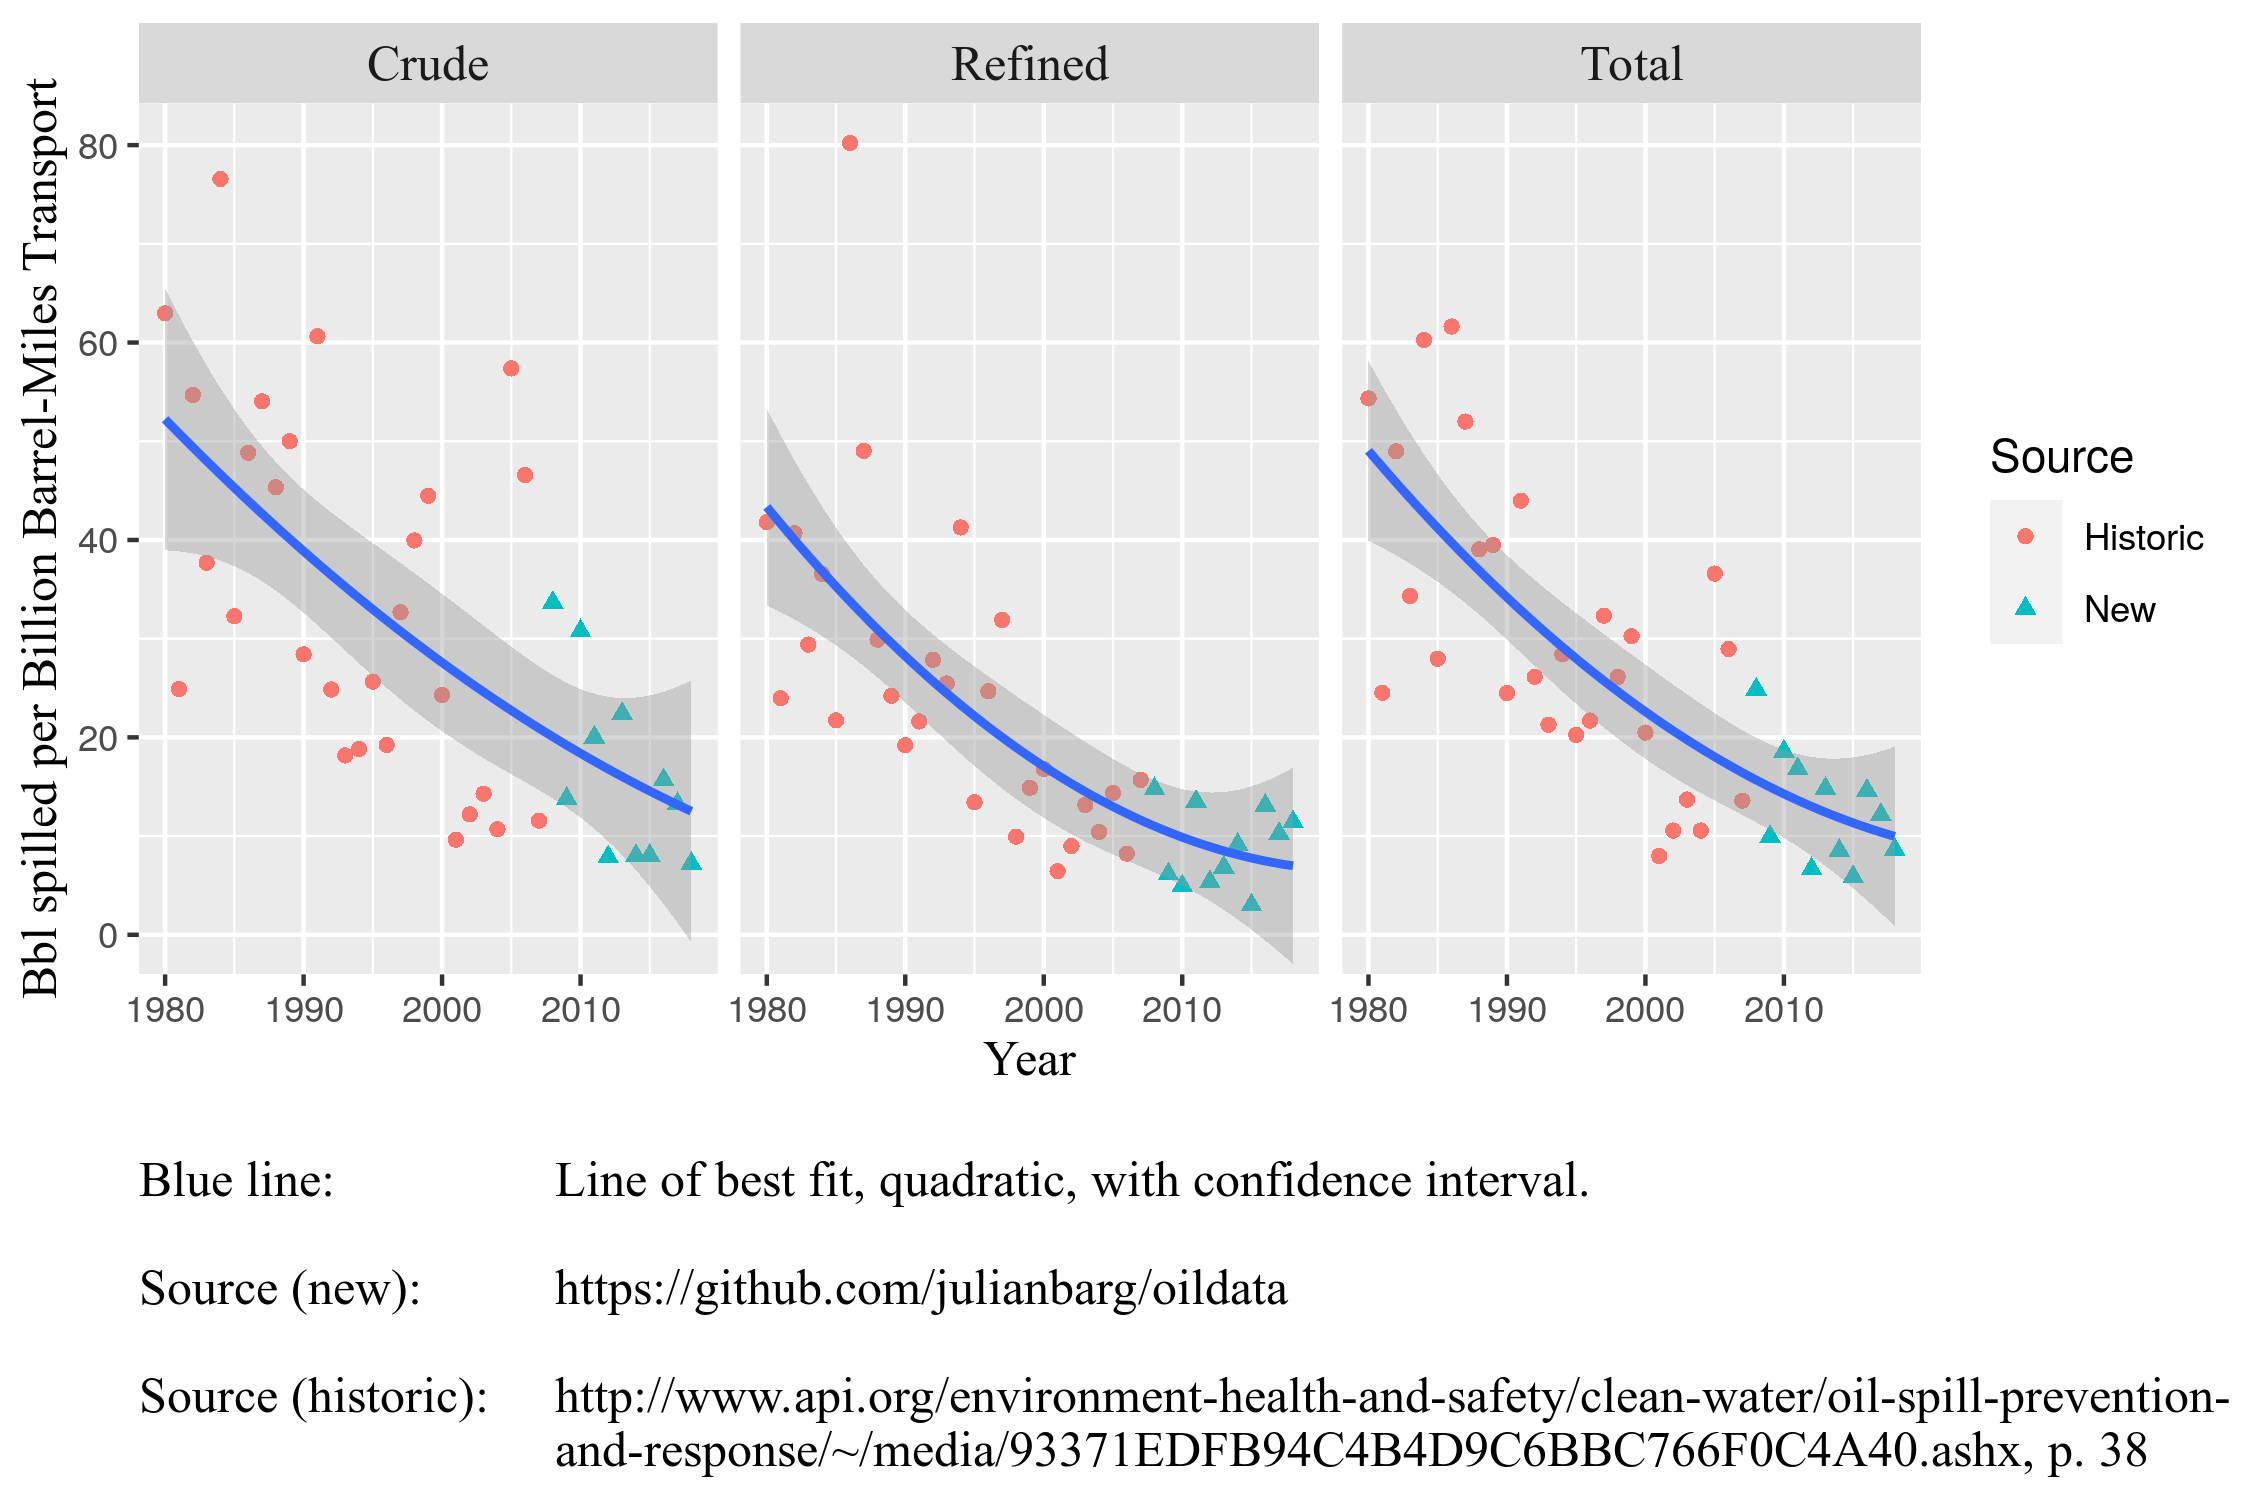
\includegraphics{../illustrations/population_learning_4.png}}
\end{figure}

Some of the findings of this dissertation might not be fully generalizable. Pipeline systems, with their manifold interactions and catastrophic potential are a great example of the complex systems and externalities discussed by \citet{Perrow1984} and citet{Beck1992}. The challenges associated with growing complexity may not be present in all other contexts. In particular, uncoupled production methods can allow for much reduced interactive potential. In these contexts, convergence of performance measures and greenwashing might take on a different shape. The complexity of pipeline systems stems from the interaction of mechanics, physics (fluid dynamics are notoriously complicated are of physics), and a complicated command structure. The diverse geography and many jurisdictions of the US also add to the complexity. In addition, there is an economic incentive to run pipeline infrastructure at a very high utilization rate and throughput, e.g., by frequently changing the commodity to be transported according to demand.\footnote{Although pipelines are generally optimized for transporting specific commodities, in principle any pipeline can transport almost any commodity when demand or supply changes.} Altogether, the complexity and interactions are not far off from what \citet{Perrow1984} observed for nuclear power plants. Many other industries constitute complex systems because of their elaborate supply chain structures, a future avenue of research would thus be whether these complex supply chains bring about the same limits to learning.

I make four contributions with this research. (1) This dissertation introduces a context where organizational learning has "bottomed out" and analyzes how learning plays out under these circumstances. The context allows us to study learning despite the absence of aggregate, quantitative improvements in performance measures because (a) we can observe the process of learning independent from the outcome in qualitative data, and (b) rich data, including textual descriptions, is available on the object of learning--individual pipeline spills. This rich data allows us to distinguish a "dynamic" state where performance measures are constant because learning and emerging challenges cancel each other out from a hypothetical "state of equilibrium" where there is no new knowledge to be obtained. Thus, this dissertation brings to the fore a state that large swaths of the learning literature have taken for granted: the "end of learning" period where performance measures make it appear as if the organization has come to a standstill. At least for this case of a complex system with catastrophic 

(2) This dissertation also makes a contribution to the discourse regarding environmental sustainability and technology. The sustainability research community is split as to the role of technology for sustainability. Some work leans more toward a technocentric view with little to no consideration of social systems, for instance in research on low-carbon electricity \citep[e.g.,][]{Greenblatt2017}. Other authors emphasize the need for changes to the political and economic system in order reduce damages to the planet, such as the degrowth discourse \citep{Kallis2018}. With regard to that debate, the findings of this research highlight the role that system complexity and unexpected externalities play for continued pollution. The pipeline industry provides a very vivid example of the limits to depolluting existing technology. Further, the greenwashing in the pipeline industry that this research surfaces should act as a cautionary tale on the role and purpose of technology in communication.

(3) This dissertation moves forward theory on learning by highlighting the considerable effort necessary to leave an existing trajectory. New knowledge needs to be created that is both valid and reliable, which requires for an organization or industry to collectively question preexisting fundamental assumptions. Applied to pipeline spills, this would imply that if society was to collectively decide that oil spills at the current level are not acceptable, then we should not rely on the industry to develop technology and make changes in the current fashion. A more fundamental rethinking of the (physical and political) system of energy delivery would be necessary.

(4) The empirical research on greenwashing highlights the potentially malevolent role that industry level organizations can play, and that technology should be taken with reservation. Actors in the pipeline industry are aware of the possibility to created a better image by creating an association between pipelines and high-tech, even in the absence of better safety performance. These actors may also be aware that is almost impossible for laymen to rebut the validity of technology that is built on decades of engineering research, and that hence the industry can safely entrench itself in this modern realm.

%The empirical sections of this dissertation use data from the US pipeline industry. Compared to other industries, both environmental pollution events and the subsequent learning process play out in a very public fashion in the pipeline industry. Large spills, which make up for a big share of the overall spill volume, are often discovered by members of the public, covered by the press, and investigated by independent government agencies. The context offers two advantages over existing empirical research. First, in the pipeline industry we can disentangle learning and the outcomes thereof. Empirical research on organizational learning commonly has to rely on improvements in performance variables to gauge learning \citep{Argote2011}. As in the context of the pipeline industry learning can be observed directly, the risk of an outcome bias is reduced \citep{Dillon2008}. The context also allows us to disentangle effective learning and rhetorics or greenwashing. In the pipeline industry, it is possible to determine when new technology and other measures are a response to existing problems, and when they are ineffective or even misleading talking points that serve to greenwash. The latter, in this specific context, is tied to industry level organizations such as the American Petroleum Institute (API) or the Association of Oil Pipe Lines (AOPL).

%This dissertation addresses two questions. (1) Can organizations that effectively learns from failures \citep{March1991} also stagnate? And (2) how does does an industry greenwash \citep{Lyon2015} this stagnation? Organization learning is observed to, after initially quick progress, converge to a certain value \citep{Argote2013-1}. In this process, organizations develop advanced, complex systems. \citet{Beck1992} and \citet{Perrow1984} suggest that unexpected interactions and externalities are intrinsic limitations of these systems. Only considerable rethinking of existing paradigms allows organizations to break out of the dead end that these complex systems can become \citep{Argyris1978, March2010, March1991}. The key to this breakout is validity and reliability of knowledge \citep{Rerup2020}. \citet{Lyon2011} suggest that instead of addressing externalities in the environmental realm, organizations may prefer to greenwash \citep{Lyon2011}. Trade associations are known to play a role in processes such as greenwashing when it occurs on a larger scale \citep{Maguire2009}.

%Between in-line inspection tools, leak detection technology, and SCADA systems that allow for the remote supervision and control of pipelines, it seems as if the pipeline industry has a technological solution to every problem thrown at it. \textit{Then why has the industry not improved its environmental performance in twenty years?} Further, if pipeline spills in the year 2020 are still common, this raises a follow-up question: \textit{How do pipeline operators regularly convince their stakeholders and the regulator that pipelines are safe}, and that they should be allowed to expand their physical footprint.


%Organizational forgetting ultimately is a routines view.
	
	\subsection{Structure}

The first chapter focuses on the empirical context, the stagnation of pipeline safety. The chapter introduces the notion of convergence in performance measures, as introduced by the \textit{learning curves} literature, which later developed into the \textit{organizational knowledge} view \citep{Argote2013-1}. This observation of convergence, which we also see in the pipeline industry, leads to the first research question, \textit{how does the convergence of performance measures take place?} One might intuitively assume that when a performance measures stay constant, no learning takes place. The qualitative data speaks to this assumption, and shows that in the pipeline industry, indeed, organizational learning still takes place. The quantitative data is then used to show that while problems are addressed with learning, new, unique problems constantly emerge. This is consistent with research on complex systems and externalities of modern technology \citep{Beck1992, Perrow1984}. Finally, the discussion section raises the alternative view, \textit{organizational routines}, and introduces the notion that a further reduction of pipeline spills requires a more radical rethinking of existing paradigms, including technology that is used. If the status quo remains as is, the research suggests that pipeline spills will continue, despite organizations learning from spills.

%begins with an orthodox view of organizational learning. Organizational learning is a useful frame for analyzing the technological side of pipeline safety, and why certain safety improvements are attained. Qualitative data reveals the learning processes taking place within the industry. The usefulness of an orthodox theory of organizational learning ends where we can observe that learning continues, but no more improvements in pipeline safety are achieved (Figure 1). The learning literature predicts this bottoming out \citep{Argote2013-1}, but does not address whether learning curves converge because learning stops, or for other reasons. This chapter examines the mechanisms behind safety improvements, the limits to learning, and the bottoming out of pipeline safety.
% Change: What matters is were trying to understand the mechanism based on empirical observations.

%The second chapter raises the issue of validity in organizational learning \citep{Rerup2020}. The current consensus is that as organizations accumulate experience from performing a task, their performance increases \citep{Argote2011}. But, as demonstrated above, one can observe an accumulation of experience with a corresponding change in cognition--a process of organizational learning--without the accompanying change in performance. Outside the literature stream on \textit{organizational knowledge} \citep{Bingham2011}, authors emphasize the ambiguity of organizational experience \citep{March2010}. This stream would contend that sometimes, to attain success, a substantial break with precedent is necessary. This chapter reunites these two disparate streams of the organizational learning literature.
% high and low intellect, second loop learning, exploration and exploitation, competency trap

The second chapter begins as a review of the organizational learning literature. The review is divided into two sections. The first section maps out the \textit{organizational knowledge} stream of the literature, including some fundamental work on \textit{learning curves}. The second section outlines the literature on \textit{organizational routines}. As a next step, the chapter turns to the fundamental difference between the two approaches. The organizational knowledge stream only recognizes learning when it occurs within the current structure--such as improvements in a specific metric--whereas the organizational routines literature recognizes radical departures as learning. These radical departures may compete with or invalidate previous insights, which represents a considerable departure from organizational knowledge stream. To reconcile the two views to some degree, the chapter finally introduces the concept of \textit{validity} and \textit{reliability} of knowledge \citep{Rerup2020}.

The third chapter turns to greenwashing this chapter returns the focus to the empirical context of the pipeline industry. After a brief introduction of greenwashing, the chapter lays out the problem at hand in the pipeline industry. Pipeline operators use new technologies in their rhetorics to assure stakeholders that pipelines are safe. This greenwashing strategy is widely shared in the industry, indicating that in this context industry level actors are also involved. The chapter uses discourse analysis to show the presence of greenwashing as a strategy across the two levels of organizations and the industry. An encompassing quantitative analysis which employs Topic Modeling to process text data \citep{Hannigan2019} then reveals how greenwashing spreads across the industry through intra-industrial networks. Finally, in the discussion section the chapter introduces the notion of technology as a vehicle for greenwashing. %Add research question?

%The third chapter discusses greenwashing as a reason why pipelines continue to fail. Despite March raising the issue of goals, coalitions, and politics in his early work \citep{March1963}, the topic is inexplicably absent from the current literature. Internal industry standards and company practice show that new insights are incorporated into practice. But the lived reality of incidents and spills is not what shapes communication with external stakeholders. Instead, in the classic greenwashing fashion, outside-facing documents are carefully crafted to convey an image of pipelines as safe and responsible, and catastrophic spills or near-spills not being the norm, but rare exceptions--the actors craft a public image \citep{Lyon2015}. For instance, to obtain a permit for the construction of a new pipeline, a pipeline operator has to establish that the pipeline is safe. Similarly, support from the public and state governments requires for pipelines to be perceived as safe. The third chapter discusses how technologies can be used in greenwashing attempts to give an industry a modern, and safe image.

	\subsection{Context and Data}

The empirical sections of this dissertation use data on the US pipeline industry. This empirical context offers a number of advantages over other datasets on environmental emissions and pollution. Compared to other industries, there is a good data coverage on pipeline spill from a diverse group of actors, including government agencies, the press, grassroot organizations, and industry level organizations. The documents on spills often include information on the events as well as causes. Further, the pipeline industry allows us to "zoom" in and out on individual oil spills and understand environmental pollution and impacts in a much more thorough fashion than is the case for other industries. Longitudinal quantitative data over a relatively long time frame is publicly available. Overall, pipeline spills as well as the subsequent learning process, and greenwashing attempts all play out in a public fashion.

Compared to environmental emissions and pollution by other industries, pipeline spills play out in a very public fashion. Pipeline spills are often initially discovered by members of the public \citep[p. 3-39]{Shaw2012}. Pipelines are built across the country, often on public land. Hence, large pipeline spills cannot rarely if ever be fully concealed from the public. Large oil spills also make up for a dominant share of the overall spill volume, hence even if some small spills are missed the data still offers an almost complete picture. When oil enters waterways, its color and smell makes the spill very obvious. Pipeline operators and employees are legally obligated to report pipeline spills.\footnote{See \url{https://www.phmsa.dot.gov/incident-reporting}, accessed 2020-08-30.} 

There are two main sources for data on pipeline spills in the US. (1) The Pipeline and Hazardous Materials Safety Administration (PHMSA) maintains a repository on all pipeline spills that occur. A fairly unique attribute of the data is that there is both qualitative and quantitative data available. Over 300 pipeline spills occur in the United States every year, and more than 100 of them are classified by the PHMSA as significant.\footnote{Meaning an injury, fire, explosion or property damage of over \$50,000, or the spill volume is at least 50bbls. See also \url{https://www.phmsa.dot.gov/sites/phmsa.dot.gov/files/docs/pdmpublic_incident_page_allrpt.pdf} and \url{https://julianbarg.shinyapps.io/incident_dashboard/}, accessed 2020-07-14.} The number of spills is sufficient for quantitative analysis to be sensible, but not at a level where an individual large spill becomes irrelevant. PHMSA also provides a dataset on pipeline operators, which allows for identification of the organization that caused each oil spills, how many miles of pipelines these organizational operate, and how much oil the organization transported over what distance each year.\footnote{See \url{https://github.com/julianbarg/oildata}, accessed 2020-07-14}. Between 2002 and 2004, PHMSA significantly increased the amount of data collected from each operator and on each spill. Hence, from 2004 forward the quality of the PHMSA data is generally good.

(2) The National Transportation Safety Board (NTSB) provides reports on pipeline spills that the agency deems significant. These reports typically have a length of 50-200 pages (usually being more than 100 pages long) and detail the incident, events leading up to it, and its causes. From 1969 until today, 142 reports and briefs have been published. The NTSB reports stand out from other reports because of the NTSB's "Go Team". Members of the Go Team are ready around the clock to be deployed to accident sites, for the benefit of collecting information that might otherwise not be available anymore.\footnote{See \url{https://www.ntsb.gov/investigations/process/Pages/default.aspx}, accessed 2020-08-31.} The NTSB also spends significant resources to determine underlying causes of (rather than liability for) the spills after the fact.\footnote{For instance, in one case NTSB tried to replicate an error of a SCADA system on a replica of the original SCADA setup \citep{NTSB2002}, and in another case NTSB used various pieces of heavy equipment on a pipeline section to determine what caused the mechanical damages that lead to a spill \citep{NTSB1990}.}

%PHMSA is the primary source for quantitative data, and NTSB the primary source for qualitative data. The NTSB reports are (obviously) biased toward very serious incidents, and the qualitative data available on less serious incidents is much less detailed. Only to some degree, this dearth of information can be counterbalanced by additional research on incidents that are not covered by NTSB, as some incidents are not reported on by any other source except for PHMSA. This lack of information on spills that are perceived as less impactful is a known limitation of research on pipeline spills. Both NTSB and PHMSA also have an overt focus on the direct impact of oil spills. The PHMSA dataset focuses on quantitative attributes of the spill, such as spill volume, volume of recovered oil, and boolean variables on remediation, whereas the NTSB focuses on the immediate impact, such as the magnitude of resulting fires, the number and types of injuries that occurred, and the immediate property damages caused. The PHMSA and NTSB data on the impact needs is supplemented with reports from residents, which both provide an understanding of the impact that the spills have on their lives, and provides a more tacit understanding of the impact on the local ecosystem. And of course the collection of third party data serves to triangulate information.

%There might either be a correlation between the \textit{complexity} of the incident and the \textit{information available} to us that is mediated by the \textit{severity} of the incident, or there could be just a correlation between the \textit{severity} of the incident and the \textit{information available}. In other words, we know whether severe incidents are more complex than less severe ones, but we do still know that they are complex.

%The qualitative and quantitative information provides us with three kinds of insights. In the first chapter, I carry out a panel regression to assess the state of organizational and population level learning in the pipeline industry. The qualitative data that is consulted indicates that specific issues are addressed through learning, but new, unique problems keep appearing, which prevents the industry from making further progress. The second chapter will not present any data, but rather discusses the learning literature while only sporadically touching on the phenomenon at hand. The third chapter uses discourse analysis and nonparticipant observation to explore the microfoundations of a coexistence of learning and a bottomed out learning curve.

In addition, other public agencies also sometimes become involved in th cleanup of pipeline spills and subsequently author reports. In addition to the quantitative data it provides, the PHMSA also occasionally commissions reports on pipeline safety \citep[e.g.,]{Shaw2012}. Other agencies that are involved with pipeline spills and provide relevant information are the Environmental Protection Agency (EPA), the National Oceanic and Atmospheric Administration (NOAA), Fire Marshals, and the coast guard. All these agencies sometimes provide primary data on the impacts of pipeline spills.\footnote{E.g., \url{https://response.restoration.noaa.gov/about/media/10-years-after-being-hit-hurricane-katrina-seeing-oiled-marsh-center-experiment-oil-clea}, accessed 2020-08-30}. Journalists also report on pipeline spills, and sometimes create very in-depth material that represents a valuable addition to government reports \citep[e.g.,][]{McGowan2012}. Finally, residents that are affected by pipeline spills sometimes organization in grassroot organizations. These grassroot organizations provide valuable data on the human impacts of pipeline spills.\footnote{E.g., \url{http://grangehallpress.com/Enbridgeblog/}, accessed 2020-08-30}.

% Paragraph on pipeline spills zoom in and out.

% Paragraph on quantitative data that is available.

%\subsection{Pipeline safety}

	\section{Literatures}

% Multiple literatures contribute to this dissertation. The challenge will be to make these languages talk to one another. The literature on \textit{Grand Challenges} provides us with a research agenda, but has little to offer (so far) that can guide our work \citep{George2015}. In lieu of input from management research on the use of natural resources, we can draw on works in interdisciplinary journals that discuss use of \textit{natural resources} by organizations \citep[e.g., ][]{Rockstrom2009}. For theory development, this dissertation builds on the learning literature. The \textit{learning literature} again falls into two camps: (1) One stream traces back to the research on \textit{learning curves}. This stream looks to disaggregate organizational learning and identify the factors that accelerate or impede learning \citep{Argote2013}. (2) The other stream originates in the \textit{behavioral theory of the firm}. That stream looks at choices and systemic impediments to learning \citep[e.g., ][]{March1963, Levitt1988, Levinthal1993}. Beyond these literatures, \textit{pipeline technology} is discussed in engineering, a stream of sociology conducts \textit{disaster research}, and research on complex systems \citep[especially][]{Perrow1984} also contributes to this dissertation. These literatures will play a subordinate role.

\subsection{Greenwashing}

Greenwashing describes a range of activities. This section provides three examples of greenwashing. This dissertation uses the third one, selective disclosure, which should be distinguished from the first two. The first, maybe the oldest one, describes an attempt of improving reputation through association with a signifier of ethics. For instance, "bluewashing" describes a corporation's effort to construe an association between a product and the United Nations \citep{Laufer2003}. 
Similarly, in marketing greenwashing describes falsely advertising a product as environmentally friendly \citep{Delmas2011}. For that purpose, a corporation does not necessarily need to make false claim. It may be sufficient to use green packaging and images of flowers. Many consumers can also be mislead with close-to-meaningless labels and certifications. 
Greenwashing has also long been a problem at the level of corporate governance \citep{Ramus2005}. With regard to environmental reporting, the term greenwashing as used in the literature often describes a process of selectively releasing positive information about one's environmental (or social) performance without also releasing negatives ones \citep{Lyon2011}. That approach of selective disclosure is insidious, because the information released are objectively true, yet, the picture of reality they paint is not accurate. The approach is also suitable for empirical research on organizations. \citet{Marquis2016} for instance operationalizes greenwashing as the difference between what share of metrics of environmental performance a corporation discloses and what share of total impacts these disclosed emissions make up for. For example, a corporation that discloses nine out of ten of its emission types, but where the missing emission type makes up for 90\% of its environmental impacts, would gain an abysmal score of $0.1 - 0.9 = -0.8$.

The abovementioned types of greenwashing have in common that none of the statements which organizations make are openly untrue, or even criminally liable. Note also that intent is not a necessary condition for greenwashing (although intent is often implied). For instance, \citet{Lyon2011} point out that a firm might itself be uncertain of its environmental impacts \citep[pp. 26f]{Lyon2011}. More universally, greenwashing can be defined as "any communication that misleads people into adopting overly positive beliefs about an organization's environmental performance" \citep[p. 225]{Lyon2015}. Within that definition, greenwashing takes on different forms. 
Since misleading communication constitutes greenwashing regardless of intent, a discussion of motivations and mechanisms for greenwashing is optional in empirical works on the topic. That definition of greenwashing as misleading communication regardless of intent describes well the developments taking place in the pipeline industry. Although the qualitative data provides several examples that suggest malicious intent, the divergence between asserted and observed pipeline safety to some degree resides at the industry level and is shared by all actors. The myth of pipelines as a safe technology is diffused at the population level by actors such as the American Petroleum Institute, the engineering profession, and shared technologies. The qualitative data allows us to make educated guesses as to the mechanisms at play at the different levels, but not to establish unambiguous intent and effect direction.

The divergence between communicated and observed pipeline safety amounts to more than just a decoupling process. The diffusion of pipeline technology ensures some coupling in the industry, and there is little evidence that technology is used throughout the industry in ways that it is not intended for. Decoupling does not equal greenwashing \citep{Lyon2015}. For example, if sustainability is decoupled in an organization because the sustainability does not have sufficient resources to effectively implement initiatives, and the organization then announces a major initiative, this communication would then qualify as greenwashing. However, not all decoupled activities result specifically in greenwashing, and not all cases of greenwashing are the result of decoupling--as mentioned above, greenwashing can also be a deliberate, malicious strategy. Decoupling could occur in other areas, such as R\&D activities, and greenwashing could result from other organizational processes, for example malice or misjudgment. This dissertation specifically discusses greenwashing that results from a technology that may function as designed, but does not deliver the results that it promises. Motives for greenwashing in this context vary. There are documents that are specifically written to testify that pipelines are safe to obtain permits \citep[e.g., discussed in][]{Stansbury2011}. But there are also grey areas, where financial interests and obligations to ensure pipeline safety are interweaved and cannot be disentangled. Decoupling certainly is not the encompassing or even dominant cause of cause of greenwashing in the pipeline industry.
	
%	\subsubsection{Chapter 1: stuff}

In chapter 1, I do amazing stuff.

	\subsection{Chapter 1: Stuck on Innovation}

	Organizational learning comes down to choices. Firms can either invest in improving existing technology, or develop new technology \citep{March1991}. Investing in the "wrong" technology can lead to technological lock-ins \citep{Levinthal1993}. The actors in the pipeline industry have selected a number of technological solutions to resolve their most pressing issue. When a pipeline spill occurs, the oil quickly infiltrates the soil and seeps into the groundwater.\footnote{The infiltration depth in sand is assumed to be over 10m in the first day alone \citep{Bonvicini2015}.} The environmental degradation caused by oil affects the local environment, and the local populace, too: a 2019 sibling comparison study on oil spills in Nigeria found that in localities that are affected by oil spills, for every 1,000 live births, an additional 38.3 neonatal deaths occur\citep{Bruederle2019}. % Potentially add impact of spills on industry? Stigmatized industry.

In their fight against pipeline spills, pipeline operators employ a variety of technologies, such as smart pigs, leak detection systems, and SCADA systems. Smart pigs, while traveling through the pipes, utilize electromagnetic flux or ultrasonic probing to assess corrosion or mechanical damages to the pipe \citep{Singh2017-7}. Internal leak detection systems measure the flow of oil at two points A and B to detect any loss in between those points. External leak detection systems detect signs of escaping hydrocarbons, and include acoustic, hydrocarbon, and temperature sensors, etc. \citep{Shaw2012}. SCADA systems are systems that allow an operator remotely monitor and operate lines. The operator typically sees on his screen charts of the flow at different points, can open and close valves, and startup or shutdown delivery of oil. Alarms from leak detection systems of the line are also displayed to the SCADA operator.\footnote{Larger pipeline companies operate control centers where all lines in a region are managed. Operators usually operate multiple SCADA systems at once, and more experienced employees supervise the operators. Control centers are operated in formal hierarchy, where for certain operations (such as clearing an alarm), a SCADA operator will require the go-ahead from a supervisor. See \citet{NTSB2012} for an in-depth description of an Enbridge control center in Edmonton as of 2012.}

The high technology character of leak detection stands in contrast to the experienced reality of pipeline spills. A 2012 study commissioned by the Pipeline and Hazardous Materials Safety Administration (PHMSA) of onshore pipeline spills that occurred over a 19 month period, SCADA systems assisted in less than 25\% of cases with the detection and confirmation of the spill \citep[p. 3-33]{Shaw2012}. In only 17\% of cases was the operator or SCADA system listed as the initial identifier of the leak, while the public or emergency responders identified 30\% of leaks \citep[p. 3-39]{Shaw2012}. Why do the great learning efforts by pipeline operators fail to deliver the safety improvements that one would expect to see? A 2012 report prepared by the National Transportation Safety Board (NTSB) on the Kalamazoo River oil spill provides a good starting point for understanding the problem. A regional manager of Enbridge is quotes as saying: "...I'm not convinced [that there is a problem]. We haven't had any phone calls. I mean it's perfect weather out here--if it's a rupture someone's going to notice that, you know and smell it" \citep[p. 100]{NTSB2012}.

Existing research has provided us with many insights on the mechanisms of organizational learning. Learning is generally regarded as a function of experience, which builds knowledge, "embedded in a variety of repositories, including individuals, routines, and transactive memory systems" \citep[p. 1124]{Argote2011}. For instance, an organization may notice that a routine fails under specific circumstances, and subsequently change its employee manual. An involved employees may also make a mental note of how to respond to the problem and whom to contact. Or an engineer might observe a method of speeding up production, and make a corresponding change to the production process. This knowledge-based approach to learning generally seeks to identify the factors that promote or hold back learning in an organization \citep[e.g.,][p. 2]{Argote2013-1}.

In terms of repositories, routines, and transactive memory systems, the pipeline industry has made great strides over our qualitative observation period. But our quantitative results do not indicate corresponding outcomes in safety improvements. The problem does not lie in a dearth of experience, or a general failure to translate "lessons" into knowledge. Our quantitative results indicate that when a specific problem occurs, the industry or individual actors are generally capable of addressing it. The coexistence of specific progress and overall stagnation is indicative of another problem.

Our qualitative analysis reveals that pipeline spills have all the hallmarks of normal accidents in complex systems \citep{Perrow1984}. Almost no two serious spills are alike, and the causes are as complex as the diverse political and physical environments that is the United States. Here, organizational learning is at an impasse. When efforts is made, and learning takes place, why do we not observe corresponding results? \citet{Levitt1988} propose that there are limitations to learning by doing. In those cases, learning cannot be disaggregated into its components. Instead, we need to look at the technological choices and determine whether an organization or industry has ended up in a competency trap \citep{Levitt1988}. An important factor for diagnosing this issue are feedback mechanisms: at the population level, is the problem diagnosed, or not? If in an industry the lack of learning goes unnoticed or is not addressed on a population level, even if learning takes place on a case-by-case basis, aggregate learning may not take place {MarchOlsen}.   

With this article, we provide an additional perspective to the learning literature. Our interpretation of the data puts into question the notion of aggregate improvements through incremental, smaller scale learning. Instead, there are more substantive, technological improvements to be made, that sometimes cannot be attained through regular learning mechanisms. In those cases, a big picture perspective on the problem or goal is necessary to made a difference.

%   Other contribution: write something on learning that fills the gap created by publication bias.

%	Hints at a problem in the learning literature. Focusing on incremental improvement.

%   Claim quantitatie data as part of initial qualitative research? We looked at 10 major spills and x years of spill data, to understand how population-level learning works. Also, claim data on population level learning as part of the research.

%	Qualitative research approach--select spills--move through spills until motives saturated.

%	Limited ability to triangulate--but that is fine because our qualitative results are quite robust, and not too complex--little chance they are wrong.

%	Another omission that we decided on for this article are flaws in the environmental feedback mechanism, akin to those predicted in \citet{March1975}. Pipeline operators are well-insulated from the consequences of their actions, as the regulator (PHMSA) is understaffed and generally gives pipeline operators the benefit of doubt [provide evidene from NTSB].


	
	\section{Chapter 3: I know that they know nothing. Knowledge and organizational learning}

\begin{singlespace}
	\begin{quote}
		"Many organizational endeavors are more dependent on the sharing of understandings (reliability) than on their correctness (validity)" -- James G. March in \textit{The Ambiguities of Experience} \citep[p. 69]{March2010}.
	\end{quote}
\end{singlespace}

Organizational learning is among the oldest of topics discussed in management research. \citet{March1963} discusses learning extensively, especially in conjunction with politics. Empirical research on learning curves goes back to the 1930s \citep{Wright1936}. Today, our understanding of the topc has reached an astounding scope \citep{Argote2013}. There exist two main views of learning. (1) The \textit{organizational routines} view describes learning as organizations developing routine responses to reoccurring scenarios. (2) The \textit{organizational knowledge} view characterizes organizations as developing a knowledge and understanding of the world, which is stored in individuals, routines, or transactive memory systems \citep{Argote2011}.

The main difference between the two approaches to organizational learning is their take on knowledge. The \textit{organizational knowledge} stream describes knowledge in relatively tangible terms. Organizations create knowledge from their experience, it is held in various different forms, and can be transferred between business units. Still, organizational knowledge in this stream \textit{is} a metaphor: the stream distinguishes between organizational knowledge and knowledge in its literal sense, as held by individuals \citep{Argote2011}. Authors in the \textit{organizational routines} stream are hesitant to allude to the concept of knowledge (1) because they are aware that organizations are not monolithic, and diverging perspectives can exist within an organization. More importantly, the second group (2) questions the capability of organizations to accurately "know" something, in light of the sparse and uncertain signals that organizations receive from the environment \citep{March1975}. This chapter discusses the concepts of \textit{validity} and \textit{reliability} of knowledge in the context of the two separate conceptualizations of organizational learning.

The ideal outcome of a discussion on organizational knowledge would be to bridge the two existing streams. That "unification" of the two streams may be difficult to achieve, because of the fundamental disagreement regarding knowledge between the two streams. Instead, this chapter introduces two concepts that at least allow for a better understanding of the fundamental rift, and maybe a partial integration. "Reliablity" describes the degree to which a piece of knowledge is shared across the members of an organization (or at another level), and validity describes whether the knowledge will enable the organization to better understand, predict, and control problems, for example technological limitations or bottlenecks \cite{Rerup2020}. On the one hand, these concepts allow for a discussion of knowledge that is compatible with the \textit{organizational routines} view. On the other hand, these concepts translate two of the main concerns raised by the the \textit{Behavioral Theory of the Firm} into the language of \textit{organizational knowledge}. Reliability talks to the political dimension of organizational behavior, and validity talks to the ambiguous nature of experience. Hence, the concepts allow for a limited integration of ideas from the two stream.

This work is motivated by events outside of the literature. Organizational learning, and especially the \textit{organizational knowledge} stream of the literature, implicitly advances a strong modernistic view of the world. To say that learning creates knowledge and can be measured in performance improvements is ultimately a tribute to enlightenment. The \textit{organizational routines} stream deviates from this formula to some extend, as it traces back its roots to research on bounded rationality \citep{March1963}. But contributors to the organizational routines stream \textit{are} also seeking to enable organizations to identify and correct their shortcomings (such as inaccurate models of the world) \citep[e.g.,][]{Argyris1978}, and ultimately are motivated by a desire for progress. Not by accident did March discuss in his last work truth, justice, and beauty--Plato's transcendentals that later became the three tenants of enlightenment \citep{March2010}. While the critical interrogation of the concept of knowledge, and the inconsistencies that this review raises may be more in line with a postmodern inquiry, the more important contribution this review is to bring attention to organizational learning where it is based on invalid or unreliable knowledge. There may be limits to an organization's ability to accurately predict the future developments on the basis of past experience, but a lack of validity and reliability has clear implications that this review alludes to. Invalid knowledge will lead to strategic actions that are much less likely to accomplish their goals--think a society that makes political decisions based on fake news. Unreliable knowledge on the other hand will lead to learning and action that is not stable--for instance the implementation of a strategy that can easily be challenged and undone by adversaries. These are the two main point that this article draws attention to.

%This literature review focuses on organizational learning. The purpose of this chapter is to shed light on the intricacies of learning in the pipeline industry from a theoretical perspective. The first section summarizes the literature of the \textit{organizational knowledge} approach. In particular, the section emphasizes the strength of the knowledge-based approach, which accurately describes the accumulation of a knowledge stock that does take place in an organization when the goal is more or less clear and the environment stable. Further, This first section summarizes some of the other accomplishments of the literature that roughly fall into the knowledge-based stream, specifically its predecessor the learning curve literature, as well as vicarious learning, and population level learning.

%The second section summarizes the \textit{organizational routines} view of organizational learning. In particular, this section highlights the gaps left by the knowledge-based approach that may be filled by work in the behavioral space. The behavioral approach appreciates the nonlinearity and messiness of learning. Significant learning can results from individuals or groups organization that seek for the organization to break with convention \citep{Argyris1978}. This form of learning poses a challenge to the knowledge-based literature, because the changes that take place fall outside the normal rubric of improvement (as exemplified by learning curves). Other examples of these qualitatively different dimensions of learning in the literature are exploration and exploitation \citep{March1991}, and high intellect vs. low intellect learning \citep{March2010}.

%Building on the review of the two approaches to learning, this literature review then discusses two critical issues, which become particularly important in the context of pipeline spills. First, in light of the leveling off of the learning curve \citep[which in the pipeline industry takes the shape of a "baseline" of spills, or "normal accidents"][]{Perrow1984}, this section addresses the merits of less complex technologies. The learning literature is implicitly technocentric, but when efficiency does not take the primacy--as is the case when dealing with toxic chemical such as oil-- rather than adding and improving technologies, scaling back and relying on less complex technologies may be a better way to go.

%Second, in light of the damages that have been brought about by the petroleum industry, it is timely to take a critical look at the modernistic assumptions of the learning literature. The learning literature should confront the fact that new technolgies also routinely bring about new problems \citep{Beck1992}. To stay with the theme of this dissertation: pipeline spills (and climate change) are problems that did not exist before the petroleum industry came into being. Acknowledging the conjunction of technology and risks is not meant to take away from the recognition of its merits. Yet, we encourage a debate about the tendency of the literature to equate "newer" with "better" rather than "different".

% multiple learning curves either fall into a learning progress toward a more abstract goal, or in a less modernistic conceptualization, learning [verb] when the organization or population turns its head toward a new goal.
	
	\section{Chapter 3: The Green Black Gold Blues. Diffusion and proliferation of greenwashing in the pipeline industry}


\begin{quote}
	Although pipeline technology has improved, new pipelines are subject to proportionally higher stress as companies use this improved technology to maximize pumping rates through increases in operational pressures and temperatures, rather than to use this improved technology to enhance safety margins. \citep[p. 4]{Stansbury2011}
\end{quote}

Like many other forms of corporate misconduct, greenwashing has been on the agenda of activists for a long time before it received the attention it deserves from the academic community\citep[e.g.,][]{Bruno1992}. Greenwashing describes "any communication that misleads people into adopting overly positive beliefs about an organization's environmental performance" \citep[p. 225]{Lyon2015}. Corporate communication with stakeholders is driven by their goals and interests. For instance, what corporations stay quiet about is as important as or more important than what they do disclose \citep{Kim2015}. Hence, what corporations say cannot be taken at face value. The greenwashing literature researches this problem. One major strategy that managers can pursue is to disclose only positive information about the environmental performance of the company, and withhold bad news \citep{Lyon2011}. To date, research has been published on this and other types of greenwashing across different industries and on various regional scales \citep{Marquis2016, Ramus2005, Seele2017, Kassinis2018}.

The existing research shows that greenwashing is a phenomenon that plays out not only at the level of individual organizations. In empirical research, to control for industry effects has become the norm \citep[e.g.,][]{Ramus2005, Marquis2016, Du2015, Testa2018}. The fact that it is necessary to control for the industry indicates that there are important processes taking place across the two levels of industry and organizations. Standards and research insights that are shared across an industry can act as templates for greenwashing, and organizations copy each other's greenwashing strategies. The greenwashing literature has yet to cover these processes. Under the watchful eye of stakeholders, entire industries such as mining, agriculture, or the energy sector have come under suspicion across the board and need to constantly put in efforts to legitimize their business models. In cases such as these, industry could even surpass organizational factors as a predictor for greenwashing. Hence, a discussion is overdue on the question: \textit{How does the industry affect organization's propensity to greenwash?}. Assisting with this question can other literature on inter-industry and cross-level processes \citep[such as][]{Maguire2009, Hardy2020}.

To empirically demonstrate the role of cross-level processes for greenwashing, this research makes use of a longitudinal dataset on pipeline safety and spills. The public repository of the Pipeline and Hazardous Materials Safety Administration (PHMSA) holds data on both individual operators' pipeline miles and the volume of crude and refined petroleum transported. Further, the repository offers a description of and quantitative data on each minor and significant pipeline spills that has occurred in the US. The analysis of text data for this research relies on Natural Language Processing (NLP)--specifically, Topic Modeling--to determine spill causes and technology trends \citep{Hannigan2019}. The descriptions of individual spills reveal the shortcomings that individual operators exhibit in terms of pipeline safety. This data is matched with text data on pipeline safety strategy obtained from annual reports or, where available, safety reports. Annual or safety reports provide insight into the strategic plans and actions of operators. Next, data on headquarter location and executives' connections (BoardEx) surfaces networks within the industry. Finally, documents by industry-level actors such as the American Petroleum Institute (API) or the PHMSA unearth the latest industry trends. Greenwashing is given where non-substantive industry trends, rather than the operator's safety problems, determine individual operators strategic plans and action. By using operators' spill frequency and volume over time, we can ensure that effective measures are not accidentally flagged as non-substantive.

By researching greenwashing in the pipeline industry in the form of non-sustantive strategic plans and actions, this research expands the greenwashing literature. The empirical analysis reveals how pipeline operators use the language of engineering and technology to divert attention from general safety issues and an industry-wide failure to reduce spill frequency and volumes, and build an image of safety and controllability. This form of greenwashing is particularly insidious, because an observer needs to first penetrate a layer of engineering and technology lingo, before the underlying issue can be surfaced. The role of industry-level actors such as the API, and an industry-wide propensity to greenwash also has clear relevance outside academic circles. Where the industry plays a role in greenwashing, policy makers and activists that seek to reign in greenwashing need to take a more systemic view, and target industry-level actors, or industries as a whole. On a related note, this unique cross-level research, which spans from the industry down to individual spills, also contributes to the literature on social-ecological systems \citep{Reyers2018}.\footnote{More recently, the need for cross-level research has also been voiced repeatedly during the ARCS Online Seminar Series and Ivey Sustainability Salon. For instance, at the Ivey Sustainability Saloon session on July 16, 2020, Tima Bansal to Nicholas Poggioli: "If the firm is at one level, one could argue that the eco-system is a different level in which many actors interact. And, arguably, Sustainable Development is a macro-level concept (system of actors)."}

%Many corporations engage in greenwashing. So what, one may say, there is always a competitor one can buy from. But not every industry has an incumbent that can be trusted to act responsible and whose products are widely available. Especially in concentrated industries, finding a "good egg" may be difficult. Greenwashing in these industries can become an issue that is pervasive, that is "part of the culture", and that is hard to eradicate. This research takes a look at one such industry where greenwashing is pervasive to understand how greenwashing spreads across this industry. From the pipeline industry, the this research generalizes to industry-wide diffusion and proliferation of greenwashing.
%
%The existing literature discusses multiple different styles of greenwashing. Their commonality is that they encompass "any communication that misleads people into adopting overly positive beliefs about an organization's environmental performance" \citep[p. 225]{Lyon2015}. Selective disclosure describes a process whereby a corporation discloses favorable information about its environmental performance, whilst withholding negative information, to attain a positive image. When implemented correctly and in the 
%absence of a harsh, reliable punishments for greenwashing the market may reward this behavior with a higher valuation \citep{Lyon2011}. Usually, it is assumed that organizations greenwash to meet stakeholder expectations, to give the impression of transparency, or simply out of opportunism \citep{Kim2015, Marquis2016}. The definition of greenwashing does not prescribe a specific mechanism that would have to be at play for an activity to qualify as greenwashing.
%
%Pipeline operators use often new and unproven technology to window dress their performance and gain permits for the construction of new pipelines. The operators advertise their use of technologies that are "safe"--that can be proven to fulfill their function in a lab setting or simulation--but that have not served to drive down the number or volume of oil spills since the turn of the millenium (see section "Introduction"). The reason for this shortcoming is that these technologies do not address the causes of spills. We will denominate these technologies in this research as not issue-oriented. The industry maintains a strong claim to safety. Pipelines, unlike oil-by-rail, are asserted to be safe, by merit of the physical principles that they operate on. Further, modern technology, as employed to improve pipeline safety, is asserted to be perfectly controllable. Typically, greenwashing in the pipeline industry falls into the realm of nonmarket strategy. This becomes most obvious when documents are specifically written to obtain a permit or attain another goal. But greenwashing is also present on corporate websites, annual reports, and publications by industry associations like the American Petroleum Institute. These documents emphasize safety initiatives, and gloss over recent spills, or emphasize spill response and remediation efforts. This myth of safe and controllable pipeline technology has also allowed the pipeline industry to attain broad public and political support in many states.\footnote{In Louisiana for example, anybody who protests on or near pipelines faces up to five years in prison, hard labor, and a \$1,000 fine. \url{https://www.propublica.org/article/how-louisiana-lawmakers-stop-residents-efforts-to-fight-big-oil-and-gas}, accessed 2020-08-19}
%
%This research takes a longitudinal approach to greenwashing and draws on data for the period form 2002 to 2019 from multiple datasets to examine greenwashing in the pipeline industry. (1) The Pipeline and Hazardous Materials Safety Administration's (PHMSA) dataset on pipeline spills and (2) on pipeline miles operated by individual operators and their utilization allows for the identification of pipeline spills and their causes. (3) Documents by the American Petroleum Institute (API) and other industry-level actors allow us to monitor the emergence of new, non-substantive technologies that fall into the realm of pipeline safety, but do not address common causes of pipeline spills. (4) Public documents by pipeline operators, such as annual reports or dedicated safety reports show the diffusion of these technologies and their use for greenwashing. (5) Data on executives in the pipeline industry, obtained from BoardEx, reveal the web of connections along which rhetorics are diffused in the industry. Finally, (6) fines levied on pipeline operators by the PHMSA, (7) post-spill statements by pipeline operators, that reveal their rational and perceived errors (albeit only ex ante), and (8) accident reports by the National Transportation Safety Board (NTSB) allow us to qualitatively assess the divergence between technological developments and spill causes.
%
%To demonstrate the degree of greenwashing in the pipeline industry, this research determines the degree to which pipeline operators' communication with the external environment is driven by industry-level trends rather than by the individual operators' recent spills. This empirical examination also gives us an understanding of how greenwashing can become commonplace in an industry. The discussion of technology that is not issue-oriented also draws attention to other forms of greenwashing that front technology but miss the issue at hand. Other example include fracking, carbon offset, and possibly carbon capture and storage. This research may also allow stakeholders and activists to better target more insidious forms of greenwashing.
%
%\subsection{Greenwashing in the pipeline industry}
%
%Greenwashing is quite common in the American pipeline industry, and the fossil fuel sector in general \citep{Kassinis2018}. The industry extensively uses the language of engineering in its rhetoric. Its communication with the outside environment is typically carried out by engineers (e.g., in feasibility studies or environmental impact analyses). American Petroleum Institute (API) engineers define standards and explores new technologies for pipeline operators. The API simultaneously lobbies against climate action. It is difficult for the "receiving side" of the communication to see through the greenwashing strategy of the pipeline industry, unless they also have specialized engineers at their disposal.\footnote{For a successful attempt, see e.g., \citet{Stansbury2011}.} The challenge is not that the claims made by engineers in the pipeline industry are factually incorrect, but that they do not address the issues that most frequently lead to pipeline spills (e.g., they involve not issue-oriented technologies). The language of engineering that documents are dressed in prevent most readers to get through to that issue
%
%By taking advantage of the language of engineering, pipeline operators gain access to a wide array of greenwashing strategies. The obvious is a stated commitment to pipeline safety, dressed in the language of engineering, but without substantiating the action to be taken. In other cases, greenwashing takes a more insidious approach, wherein the language of engineering and pipeline safety will conceal the primacy of business interests. For instance, the language and engineering can be used to misrepresent investments with a financial interests as primarily motivated by safety, or to obtain objectively verifiable data that cannot be refuted by stakeholders that are laymen. The following are two examples: (1) after a 2010 oil spill that polluted the Kalamazoo River in Michigan, Enbridge agreed to spend at least \$110 Million to improve pipeline safety.\footnote{\url{https://archive.epa.gov/epa/newsreleases/united-states-enbridge-reach-177-million-settlement-after-2010-oil-spills-michigan-and.html}, accessed 2020-08-19.} Enbridge successfully translated this settlement into an investment by using the money to increase its pipeline capacity and transport more oil along the same route. The residents that had been affected by the spill lost out against Enbridge a second time: once again they had their lifes disrupted, this type by construction work in their backyard, sometimes on a very short notice. Enbridge successfully circumvented the need for an environmental impact assessment by replacing the pipeline in short sections.\footnote{For brief summary of events, see \url{https://www.youtube.com/watch?v=IAR7z76KWj8}, accessed 2020-08-08.}
%
%(2) In 2006, in a confidential document that was later leaked, a consulting company on behalf of the TransCanada Corporation made two claims. If the Keystone Pipeline was to be constructed the operator could using the latest technology detect a large spill in as little as 9 minutes, and any spill over 50 barrels would only occur once every seven years \citep{Consulting2006}. This claim was not testable at the time but did convince the regulator to greenlight the construction of the pipeline. The pipeline began operation in 2010, and as of 2020 had experienced 5 spills of over 50 barrels,\footnote{See \url{http://boldnebraska.org/keystone-pipeline-spill-history/}, or \url{https://julianbarg.shinyapps.io/incident_dashboard/}, accessed 2020-08-08.} including one case where the spill continued for 20 minutes after the affected landowner who had discovered the spill had called in\footnote{\url{https://www.thedickinsonpress.com/business/energy-and-mining/4004561-5-years-after-spill-rancher-and-pipeline-junkie-still-has}, accessed 2020-08-08}. The problems of the Keystone Pipeline are symptomatic of spill detection technology: a sensitive system can detect small spills but will also produce many false positives. Thus, the real challenge is actually the far more complex one of managing the safety culture, since personnel can easily become desensitized by frequent false alarms and even safety drills.\footnote{See e.g., \url{https://www.ntsb.gov/investigations/AccidentReports/Reports/PAR1201.pdf}, p. 101.} For a discussion of the role of the consulting firm in misleading the regulator in that case, see \citet{Stansbury2011}.
%
%\section{Assessing greenwashing in the pipeline industry}
%
%In order to empirically assess greenwashing in the American pipeline industry, this research focuses on two kinds of greenwashing. The first is non-substantive promises made. These are commitments to pipeline safety without details on action, or without the organization following through. This version of greenwashing can be coded by hand, as long as comparable documents are available across time. The second aspect are technologies that are not issue-oriented. Referrals to these technologies, we can capture by using Natural Language Processing (NLP): either through keyword searches, or by utilizing topic modeling.
%
%Since the quality of the text data will be the key to obtaining meaningful results, constructing a good sample is of the essence. A list of the largest pipeline operators can be extrapolated from the Pipeline and Hazardous Materials Safety Administration (PHMSA) dataset. To obtain good quality text data, my sampling strategy focuses on the largest players in the industry, and completeness across time. Where annual reports or similar documents cannot be obtained from central sources such as Mergent Archives, the SEC, or \url{www.annualreports.com}, the documents are collected as much as possible by hand from corporate websites. For the empirical section of this research, the two different types of greenwashing (non-substantive and technology-based) are tracked across organizations and across time. We obtain evidence that teh communication does in fact constitute greenwashing by comparing the diffusion of technology in rhetorics with actual spill rates and volumes. The empirical test then shows that the communication with the external environment on pipeline safety is determined by networks of diffusion for greenwashing much more than by recent failure modes, by substantive safety issues that could be addressed. To show that mismatch between communication and issues, this research takes advantage of both non-substantive communication and of the different types of technologies that are applied but that are not issue-oriented. These types of greenwashing we can track across the company documents and industry-level documents, and compare that data to the network data available from BoardEx. The importance of industry-level actors comes even more into focus when we turn to instances of deregulation in Louisiana and Texas. These instances of deregulation should act as exogenous shocks for greenwashing. We can expect that following these exogenous shocks the share space given to technologies that are not issue-oriented or non-substantive communication should become even more widespread.
	
%		\section{Conclusion}
	\begin{itemize}
		\item Reliability and validity: could look into that for answers/solutions.
		\item What areas of \citet{George2016} are not covered? I will pick those off in future research and could set that up here.
		\item Limitation: assuming that spills encompassing.
	\end{itemize}

% 	\input{sections/timeline}

\bibliography{bibliography}

\end{document}